\documentclass[12pt,a4paper]{article}
\usepackage[UTF8]{ctex}
\usepackage{amsmath,amssymb}
\usepackage{xcolor}
\usepackage{hyperref}
\usepackage{geometry}
\usepackage{graphicx}
\geometry{margin=2.5cm}

\title{Quantum Integer / 量子整数}
\author{QuoNic}
\date{}

\begin{document}
\maketitle

\begin{center}
\textbf{Language / 语言特性} | 难度：初级 | 预计时间：5 分钟
\end{center}

\tableofcontents
\newpage

\section{为什么需要？}

量子整数是量子程序中的整数数据类型。

\subsection{经典局限}
\begin{itemize}
  \item 经典整数无法直接用于量子态
  \item 需要量子编码
\end{itemize}

\subsection{量子优势}
\begin{itemize}
  \item 量子整数可以在量子程序中使用整数操作
  \item 是量子数据类型的基础
  \item 支持量子算术运算
\end{itemize}

\subsection{实际应用}
\begin{itemize}
  \item 量子算术
  \item 量子编码
  \item 量子算法设计
\end{itemize}

\section{快速上手}

\begin{verbatim}
from quonic import qint

# 量子整数
a = qint(3, n_bits=4)
b = qint(5, n_bits=4)
c = a + b
print(f'Result: {c}')
\end{verbatim}

\textbf{预期输出}：
\begin{verbatim}
Result: 8
\end{verbatim}

\section{原理详解}

\subsection{电路图}

\begin{center}
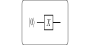
\includegraphics[width=0.6\textwidth]{../../images/qint_circuit.svg}
\end{center}

\subsection{数学推导}

量子整数编码：
\begin{equation}
|n\rangle = |b_{k-1} b_{k-2} \ldots b_1 b_0\rangle
\end{equation}

其中 $b_i$ 是二进制位。

\textbf{量子加法}：
\begin{equation}
|a\rangle|b\rangle \to |a\rangle|a+b\rangle
\end{equation}

\subsection{几何解释}

量子整数在计算基态中编码整数值。量子算术运算通过量子门实现。

\section{代码详解}

\begin{verbatim}
from quonic import qint

# qint(value, n_bits)
# value: 整数值
# n_bits: 量子比特数

a = qint(3, n_bits=4)  # |0011>
b = qint(5, n_bits=4)  # |0101>

# 量子加法
c = a + b
print(f'Result: {c}')  # 8
\end{verbatim}

\section{进阶用法}

\subsection{场景 1：量子算术}

\begin{verbatim}
from quonic import qint

# 量子算术
a = qint(3, n_bits=4)
b = qint(5, n_bits=4)

# 加法
c = a + b
print(f'{a} + {b} = {c}')

# 乘法
d = a * b
print(f'{a} * {b} = {d}')
\end{verbatim}

\subsection{场景 2：量子编码}

\begin{verbatim}
from quonic import qint

# 量子编码
data = [1, 0, 1, 1]
encoded = qint(data, n_bits=4)
print(f'Encoded: {encoded}')
\end{verbatim}

\section{适用场景}

\subsection{量子算术}

量子整数用于量子算术运算。例如，量子加法、量子乘法等。

\subsection{量子编码}

量子整数用于量子编码。例如，将经典数据编码为量子态。

\section{常见问题}

\subsection{量子整数和经典整数有什么区别？}

量子整数在量子态中编码，经典整数在经典变量中存储。量子整数可以处于叠加态。

\subsection{量子整数的精度如何？}

精度取决于量子比特数。更多的量子比特提供更高的精度。

\section{学习路径}

\subsection{前置知识}
\begin{itemize}
  \item 量子比特
  \item 量子门
  \item 量子测量
\end{itemize}

\subsection{继续学习}
\begin{itemize}
  \item 量子算术
  \item 量子编码
  \item 量子算法设计
\end{itemize}

\section{完整示例代码}

\subsection{示例 1：基本量子整数}

\begin{verbatim}
from quonic import qint

a = qint(3, n_bits=4)
b = qint(5, n_bits=4)
c = a + b
print(f'Result: {c}')
\end{verbatim}

\section{下载}

\begin{itemize}
  \item [qint.py](https://github.com/ChrisLee0721/QuoNic/blob/main/examples/qint/qint.py)
\end{itemize}

\end{document}
